%!TEX root = ../template.tex
%%%%%%%%%%%%%%%%%%%%%%%%%%%%%%%%%%%%%%%%%%%%%%%%%%%%%%%%%%%%%%%%%%%%
%% F2_stateoftheart.tex
%% NOVA thesis document file
%%
%% Chapter with lots of dummy text
%%%%%%%%%%%%%%%%%%%%%%%%%%%%%%%%%%%%%%%%%%%%%%%%%%%%%%%%%%%%%%%%%%%%

\typeout{NT FILE F2_stateoftheart.tex}%


%%%%%%%%%%%%%%%%%%%%%%%%%%%%%%%%%%%%%%%%%%%%%%%%%%
\chapter{Estado da Arte}
\label{cha:estado_da_arte}
%%%%%%%%%%%%%%%%%%%%%%%%%%%%%%%%%%%%%%%%%%%%%%%%%%



%%%%%%%%%%%%%%%%%%%%%%%%%%%%%%%%%%%%%%%%%%%%%%%%%%
\section{Redes NDN}
\label{sec:redes_NDN}
%%%%%%%%%%%%%%%%%%%%%%%%%%%%%%%%%%%%%%%%%%%%%%%%%%
No início, quando as ideias centrais que fundamentaram a Internet começaram a ser desenvolvidas, a solução de comunicação oferecida pelo TCP/IP fosse única e revolucionária, o problema que ela resolveu era essencialmente o de conversas ponto a ponto entre duas entidades. Apesar de o TCP/IP ter sido concebido para conversos entre pontos finais de comunicação, acabou por superar todas as expectativas sendo também amplamente utilizado na distribuição de conteúdo, levando assim a Internet a passar a funcionar como uma rede de distribuição. Sendo assim tornou-se muito difícil resolver problemas pois as redes de distribuição são mais complexas que as redes de comunicação. A natureza do IP está implementada nos seus datagramas, identificando apenas os pontos iniciais e finais de comunicação. O \gls{NDN} propõe generalizar a arquitetura da Internet, removendo essa limitação pois os nomes de um datagrama \gls{NDN} passam a ser estruturados hierarquicamente, sendo que podem ser utilizados para identificar um pedaço de dados dentro de uma conversa ou um pedaço de conteúdo. Esta mudandça, teoricamente simples, permite que se resolva uma alta gama de problemas de distribuição. A comunicação \gls{NDN} é impulsionada pelos recetores, existindo apenas 2 pacostes: os pacotes de interesse e os pacotes de dados (Figura \ref{fig:Packets}).
\begin{figure}[h]
    \centering
    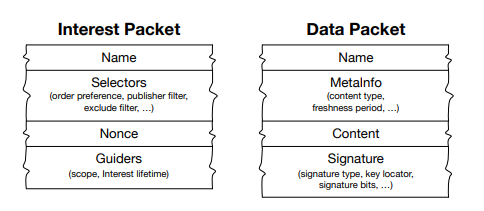
\includegraphics{Chapters/Figures/Packets.png}
    \caption{Pacotes das redes \gls{NDN} \cite{papadopoulos_lixia_2014}}
    \label{fig:Packets}
\end{figure}
O consumidor coloca o nome da parte dos dados desejada no pacote de interesse e envia-o para a rede, os routers usam o o nome para encaminhar o interesse em direção aos produtores dos dados. Quando o interesse chega ao nó que possui os dados solicitados, esse nó retornará um pacote de dados que contém o nome e o conteúdo. Este pacote segue on caminho inverso ao caminho percorrido pelo pacote de interesse.

%%%%%%%%%%%%%%%%%%%%%%%%%%%%%%%%%%%%%%%%%%%%%%%%%%
\subsection{\emph{Funcionamento do \gls{NDN}}}
\label{sub:func__NDN}
%%%%%%%%%%%%%%%%%%%%%%%%%%%%%%%%%%%%%%%%%%%%%%%%%%

Para realizar as funções de encaminhamento de intersses e dados, os routers \gls{NDN} matém três estruturas: as \gls{PIT}, as \gls{FIB} e as \gls{CS}.
A \gls{PIT} é uma tabela que armazena todos os interesses que ainda não foram satisfeitos. Cada entrada regista o nome dos dados, juntamente com as interfaces de entrada e de saída. Quando chega um pacote de interesse, o router verifica a \gls{CS} procurando os dados correspondentes, se existirem o pacote de dados é logo retornado pela mesma interface pela qual chegou o interesse. Caso contrário, o router procura o nome na \gls{PIT}, e se uma entrada correspondente existir, regista a interface de entrada na tabela.
Se na \gls{PIT} não houver nenhuma entrada correspondente ao nome, o router encaminha os dados ao produtor com base nas informações da sua \gls{FIB}, bem como na estratégia de encaminhamento. Este processo pode ser visto na Figura\ref{fig:Forwarding}.

\begin{figure}[h]
    \centering
    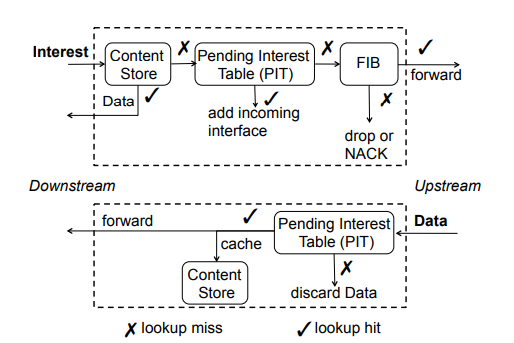
\includegraphics{Chapters/Figures/fowarding.png}
    \caption{Processo de encaminhamento num nó \gls{NDN} \cite{papadopoulos_lixia_2014}}
    \label{fig:Forwarding}   
\end{figure}

Quando um router recebe interesses para o memsmo nome de multiplos nós ele vai apenas encaminhar aenas o primeiro em direção ao produtor de dados. A \gls{FIB} é populada por um protocolo baseado no prefixo de nome e pode ter várias interfaces de saida para cada prefixo. A estratégia de encaminhamento pode decidir descatar um interesse em algumas situações, um exemplo, é se todos os links estiverem cosgestionados ou em caso de suspeição de ataque. Para cada interesse, a estrategia de encaminhamento recupera a entrada correspondente ao prefixo mais longo da \gls{FIB} e decide quando e para onde encaminhar os interesses. O \gls{CS} é uma memória \textit{cache} temporária de pacotes de dados recebidos pelo router. Como um pacote de dados \gls{NDN} é independente de onde vem ou para onde vai, pode ser armazenado em cache para satisfazer futuros interesses. Quando chega um pacote de dados, o router \gls{NDN} encontra a entrada na \gls{PIT} e encaminha os dados para todas as interfaces nessa entrada, após isso remove essa \gls{PIT} e armazena os dados na \gls{CS}. Para grandes objetos de conteúdo que compreendem vários pacotes, os interesses desempenham um papel importantíssimo no controlo de fluxo como os \textit{ACKs} do TCP. Nem os pacotes de interesse nem os de dados transportam endereços, os routers encaminham os pacotes de dados com base nos nomes contidos nos pacotes e encaminham pacotes de dados para os consumidores com base nas informações de estado da \gls{PIT} configuradas em pelos interesses em cada salto. Essa simetria na troca dos pacotes interesse7dados induz um loop de controlo \textit{hop-by-hop}, e elimina a necessidade de qualquer noção de nós.

%%%%%%%%%%%%%%%%%%%%%%%%%%%%%%%%%%%%%%%%%%%%%%%%%%
\section{\emph{Sincronização no \gls{NDN}}}
\label{sub:Sinc__NDN}
%%%%%%%%%%%%%%%%%%%%%%%%%%%%%%%%%%%%%%%%%%%%%%%%%%
O objetivo da sincronização no \gls{NDN} é reconciliar as diferenças num conjunto de dados partilhado entre múltiplos participantes, ou seja, com o conhecimento de todos os dados disponíveis os utilizadores podem decidir quando e se recuperar dados em falta. À medida que novos dados são gerados pelos produtores, é essencial que os mebors sejam informados sobre alterações. Cada utilizador transmite o seu Estado para os outros pariticipantes através de trocas de Interesse-Dados. Esta troca pode ser feita de duas forma, o produtor notificar ativamente sobre o seu estado, ou cada utilizador consultar periodicamente o grupo de sincronização.
Uma abordagem para a reconciliação dos dados é o uso de vetores de estado. A ideia central é representar o estado de um conjunto de dados na forma de um vetor de versão, onde cada componente corresponde ao nome mais recente dos dados de cada produto. Como um vetor de estado enumera diretamente o prefixo de cada produtor e o número de sequência dos dados mais recentes, as diferenças nos conjuntos de dados podem ser identificadas fazendo uma simples comparação entre os valores de cada prefixo. Para atualizar o seu Vetor de Estado, o nó adota o maior numéro de sequência disponível para cada produtor. O facto de a representação do estado baseada em Vetores de Estado permitir uma comparação direta do estado, permite que os nós identifiquem diretamente os dados em falta sem necessidade de trocas de mensagens adicionais. Esta característica torna a abordagem ideal para redes ad-hoc, onde grandes divergências de estado são bastante comúns. O tamanho do Vetor cresce proporcionalmente ao número de produtores cujos estados precisam ser trocados. Contudo, a listagem explícita dos estados de cada produtor permite a transmissão de Vetores de Estado parciais quando há restrições no tamanho dos pacotes.
Como um Vetor de Estado enumera diretamente o prefixo do produtor e o número de sequência dos dados mais recentes para cada produtor em um grupo de Sincronização, conforme mostrado na Figura \ref{fig:SV}, a diferença nos nomes dos conjuntos de dados pode ser identificada diretamente comparando o número de sequência de cada prefixo de produtor. Em seguida, um nó atualiza seu Vetor de Estado adotando o valor mais alto do número de sequência de cada produtor no Vetor de Estado.

\begin{figure}[h]
    \centering
    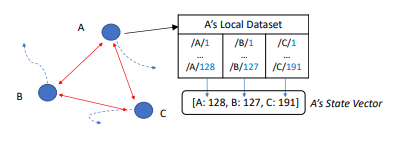
\includegraphics{Chapters/Figures/svs.png}
    \caption{Exemplo de Vetor de Estado \cite{li_brief_2018}} 
    \label{fig:SV}   
\end{figure}

Como o NDN foi concebido para suportar comunicações assíncronas, exigir uma consistência perfeita das informações de associação entre todos os membros do grupo não é viável. Para contornar esta limitação, o sincronização por Vetores de Estado foi rapidamente sucedida por outro protocolo de sincronização, o DSSN. O DSSN trouxe uma alteração simples, mas crucial, permitindo a sincronização de conjuntos de dados em grupos de sensores que entram periodicamente em estados de inatividade.
A principal mudança introduzida pelo DSSN foi a reformulação do vetor de estado, que passou de uma simples lista de números de sequência para uma lista de tuplas [prefixo-do-participante, número de sequência]. Com este novo formato, cada Interesse de Sincronização do DSSN transporta um vetor de estado que codifica diretamente o estado global do conjunto de dados partilhado. Esta abordagem garante que qualquer destinatário pode interpretar corretamente a mensagem DSSN, independentemente do nível de inconsistência de estado entre os participantes.
O DSSN foi projetado para ambientes onde a conectividade entre nós fixos é intermitente. A partir deste protocolo, surgiu o DDSN, uma extensão do DSSN otimizada para redes ad hoc sem fio, caracterizadas por uma alta dinâmica no movimento dos nós. Para lidar com estas condições, o DDSN introduziu uma série de melhorias, incluindo:

\begin{itemize}

    \item 1. Priorização de transmissão que permite determinar quais mensagens devem ser enviadas primeiro durante períodos de conectividade transitória.

   \item  2. Modo inativo que reduz o tráfego de sincronização e otimiza o consumo de energia quando não há outros nós dentro da área de comunicação.
\end{itemize}
Apesar da sua eficiência em ambientes altamente dinâmicos e disruptivos, o DDSN tem um desempenho inferior em redes bem conectadas, devido à sua ênfase exclusiva em cenários com conectividade instável. A experiência adquirida com os protocolos anteriores levou ao desenvolvimento do \gls{SVSync}. Este protocolo herda a codificação do vetor de estado introduzida pelo DSSN, mas elimina funcionalidades específicas para redes de sensores e ambientes com elevada disrupção.

%%%%%%%%%%%%%%%%%%%%%%%%%%%%%%%%%%%%%%%%%%%%%%%%%%
\subsection{\emph{\textit{State Vector Sync} \gls{SVSync}}}
\label{sub:Sinc__NDN}
%%%%%%%%%%%%%%%%%%%%%%%%%%%%%%%%%%%%%%%%%%%%%%%%%%

O \gls{SVSync} adota uma estratégia de codificação de estado distinta. O seu design segue a convenção de nomeação sequencial dos dados e transporta diretamente a representação do namespace do conjunto de dados, codificada em pares [nome do produtor, número de sequência] (figura \ref{fig:SVs}), dentro de cada Interesse Sync Multicast.
A decisão de design do SVS de incluir o namespace do conjunto de dados bruto em cada Interesse de Sincronização oferece uma vantagem significativa: qualquer nó que receba o Interesse compreende de imediato o estado do conjunto de dados, independentemente do seu próprio estado atual ou de eventuais mensagens perdidas anteriormente. No entanto, permitir que um Interesse recebido possa alterar o estado de um participante abre a porta a possíveis abusos. Para mitigar esse risco, o SVS exige que todos os Interesses de Sincronização sejam assinados.

\begin{figure}[h]
    \centering
    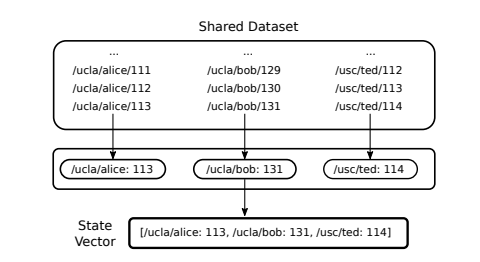
\includegraphics{Chapters/Figures/vsvsync.png}
    \caption{Exemplo de Vetor de Estado \cite{moll_brief_nodate}} 
    \label{fig:SVs}   
\end{figure}

\subsubsection{Funcionamento do \gls{SVSync}}
Um grupo de sincronização utiliza um prefixo multicast de grupo, garantindo que todos os participantes recebem as mensagens de sincronização. Cada membro do grupo possui também um prefixo de publicação específico, sob o qual os seus dados ficam acessíveis aos outros participantes.
O \gls{SVSync} opera com apenas um tipo de mensagem: o Interesse de Sincronização, utilizado para atualizar o estado do conjunto de dados. Estes Interesses de Sincronização são enviados para o prefixo multicast de grupo em duas situações:
\begin{itemize}
    \item 1. Acionados por eventos, sempre que há uma alteração no estado do conjunto de dados, os participantes notificam imediatamente os restantes.
    \item 2. Envios periódico, garantem uma visão consistente do conjunto de dados, mesmo em caso de perda de mensagens acionadas por eventos.
\end{itemize}
O primeiro caso é utilizado para disseminar rapidamente novas informações sobre o estado do conjunto de dados na rede, enquanto o segundo serve para garantir a consistência do estado do conjunto de dados do grupo, mesmo perante perdas de pacotes e desconexões temporárias.
Os interesses de sincronização ativados por eventos garantem que o grupo se mantém atualizado sobre o estado do conjunto de dados partilhado. No entanto, o estado de um determinado membro pode ficar desatualizado em relação aos restantes devido a diversas razões imprevisíveis, como perda de pacotes ou falhas temporárias de ligação. Para mitigar este problema, cada entidade de sincronização mantém um temporizador de interesse de sincronização para acionar periodicamente esses interesses, ajudando a manter os membros do grupo sincronizados.
O funcionamento desse mecanismo é explicado na figura \ref{fig:SVsyync}.

\clearpage
    \begin{figure}[h]
        \centering
        \includegraphics{Chapters/Figures/Captura de ecrã 2025-03-24 160649.png}
        \caption{Fluxograma do funcionamento do \gls{SVSync} \cite{moll_brief_nodate}} 
        \label{fig:SVsyync}   
    \end{figure}

    Diferindo dos protocolos anteriores baseados em vetores, os interesses de sincronização \gls{SVSync} são utilizados exclusivamente como notificações unidirecionais, sem desencadear pacotes de resposta. Todos os protocolos de sincronização utilizam interesses de sincronização para transmitir o estado do conjunto de dados, diferenciando-se apenas na forma como codificam esse estado.
    Os participantes de um grupo de sincronização transmitem interesses de sincronização multicast para todo o grupo. No entanto, solicitar notificações de mudança de estado através de interesses multicast levanta três desafios principais:
    \begin{itemize}
        \item 1. Como o momento da próxima alteração no estado do conjunto de dados é imprevisível, um interesse de sincronização que solicite uma resposta permanecerá pendente em todos os nós encaminhadores até expirar e ser renovado. Isto cria um estado PIT persistente para cada membro relativamente a todos os outros membros do grupo.
        \item 2. Um interesse multicast solicita uma resposta de vários produtores potenciais. Se múltiplos produtores responderem quase simultaneamente, devido ao princípio do NDN de um interesse-um dado, apenas uma das respostas será entregue ao remetente do interesse.
        \item 3.	Como consequência do ponto anterior, diferentes membros do grupo poderão receber atualizações distintas, levando a uma divergência do estado do conjunto de dados, que só convergirá após vários ciclos de troca de interesse-dado.
    \end{itemize}
    Para resolver estes problemas, em vez de solicitar respostas diretamente através de interesses de sincronização multicast, o \gls{SVSync} utiliza-os apenas para permitir que cada participante notifique os restantes sobre o seu próprio estado do conjunto de dados. 
